\documentclass[11pt,border=5pt]{standalone}
\usepackage{fontspec}
\setmainfont{cmunrm.otf}[BoldFont=cmunbx.otf,ItalicFont=cmunti.otf,BoldItalicFont=cmunbi.otf]
\usepackage{amsmath}
\usepackage{unicode-math}
\setmathfont{NewCMMath-Regular.otf}
\usepackage{tikz}
\usetikzlibrary{arrows.meta,patterns,angles,quotes}
\begin{document}
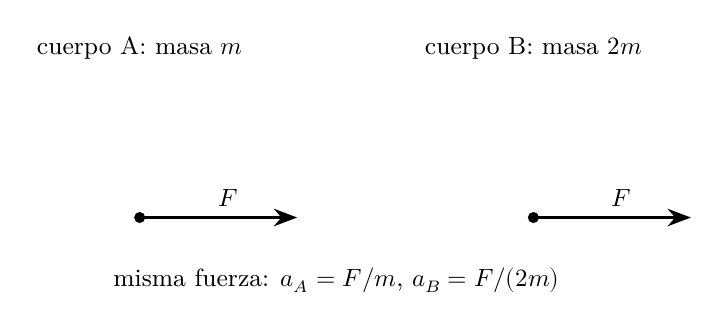
\begin{tikzpicture}[>=Stealth,font=\small,line cap=round,line join=round]
\fill (0,0) circle (2pt);
\draw[->,very thick] (0,0) -- (2,0) node[pos=0.55,above] {$F$};
\node at (0,2.15) {cuerpo A: masa $m$};
\begin{scope}[xshift=5cm]
\fill (0,0) circle (2pt);
\draw[->,very thick] (0,0) -- (2,0) node[pos=0.55,above] {$F$};
\node at (0,2.15) {cuerpo B: masa $2m$};
\end{scope}
\node at (2.5,-0.8) {misma fuerza: $a_A=F/m$, $a_B=F/(2m)$};

\end{tikzpicture}
\end{document}
